\documentclass[xcolor=dvipsnames]{beamer}
\usepackage{lmodern}
\usepackage[T1]{fontenc}
\usepackage[english]{babel}
\usepackage[utf8]{inputenc}

\usepackage{manfnt}
\usepackage{wasysym}
\usepackage{listings}
\usepackage{graphicx}
\usepackage{url}
\usepackage{ulem}
\usepackage{marvosym}
\usepackage{proof}
\usepackage{array}
\setbeamertemplate{navigation symbols}{}

\title[Demystifying Debugging]{{\bf Demystifying Debugging}}
\subtitle[]{{\em when getting it right the first time every time fails}}
\author[Ben Blum]{Ben Blum \texttt{(bblum@andrew.cmu.edu)}}

\institute[98-172]{Great Practical Ideas for Computer Scientists}
\date[]{2012, November 8}

\setbeamertemplate{footline}{\hspace*{.5cm}\scriptsize{\insertauthor\hspace*{50pt} \hfill\insertframenumber\hspace*{.5cm}}}

\usecolortheme{seahorse}
\usecolortheme{rose}
\useoutertheme{infolines}

\usecolortheme[named=RoyalBlue]{structure}

\newcommand\noob{\mathsf{noob}}
\newcommand\gibs{\mathsf{gibs}}
\newcommand\dps{\mathsf{dps}}
\newcommand\squig\rightsquigarrow
\newcommand\Coloneqq{\mathrel{\mathop{::}}=}
\newcommand\dmg{\text{\Laserbeam}}
\newcommand\delter\delta
\newcommand\alpher\alpha
\newcommand\defnor{\text{ }|\text{ }}

\newcommand\pimp{\mathop{\supset}}
\newcommand\pand{\mathop{\wedge}}
\newcommand\por{\mathop{\vee}}
\newcommand\ptrue{\top}
\newcommand\pfalse{\bot}


\begin{document}
% \renewcommand{\inserttotalframenumber}{28} % If you want to hide bonus slides
\normalem
\begin{frame}
	\titlepage
\end{frame}

%%%%%%%%%%%%%%%%%%%%%%%%%%%%%%%%%%%%%%%%%%%%%%%%%%%%%%%%%%%%%%%%%%%%%%%%%%%%%%%%
%%%%%%%%%%%%%%%%%%%%%%%%%%%%%%%%%%%%%%%%%%%%%%%%%%%%%%%%%%%%%%%%%%%%%%%%%%%%%%%%
%%%%%%%%%%%%%%%%%%%%%%%%%%%%%%%%%%%%%%%%%%%%%%%%%%%%%%%%%%%%%%%%%%%%%%%%%%%%%%%%

\newcommand\linegap{\vspace{0.2in}}
\newcommand\breakslide[1]{\begin{frame}{} \begin{center} \Large #1 \end{center} \end{frame}}
\newcommand\related[1]{\textsuperscript{\em [#1]}}
\newcommand\hilight[2]{\color{#1}#2\color{black}}
\definecolor{grey}{RGB}{127,127,127}
\definecolor{darkcyan}{RGB}{0,127,127}
\definecolor{olivegreen}{RGB}{0,127,0}
\definecolor{violet}{RGB}{127,0,127}
\definecolor{brickred}{RGB}{127,0,0}
\definecolor{brown}{RGB}{127,63,0}


\begin{frame}{Outline}
	\textbf{Why teach debugging?}
		% brief motivation
		% toolbox
	\linegap

	\textbf{``Tell Me a Story''}
	\begin{itemize}
		\item The good debugger's attitude
			% "get more operators"
		\item Binary Search
	\end{itemize}
	\linegap

	{\bf Two Main Approaches}
	\begin{itemize}
		\item Time Travel
			% small test cases / minimize the test case
		\item Space Travel
			% printf debugging
			% invariant checkers and asserts
	\end{itemize}
	\linegap

	{\bf Assorted Tricks}
	\begin{itemize}
		\item Question assumptions
		\item Collect data
	\end{itemize}
\end{frame}

%%%%%%%%%%%%%%%%%%%%%%%%%%%%%%%%%%%%%%%%%%%%%%%%%%%%%%%%%%%%%%%%%%%%%%%%%%%%%%%%
\section{Motivation}
%%%%%%%%%%%%%%%%%%%%%%%%%%%%%%%%%%%%%%%%%%%%%%%%%%%%%%%%%%%%%%%%%%%%%%%%%%%%%%%%

\begin{frame}{``The Universal Backup Plan''}
	\textbf{15-112, 15-122, 15-150, ...}
	\begin{itemize}
		\item What do these classes all have in common?
		\pause
		\item How to write code that {\em works}
	\end{itemize}
	\pause
	{\bf 98-172}
	\begin{itemize}
		\item What to do with code that {\em doesn't}
	\end{itemize}
	% TODO: a picture goes here -- blank slate vs equipped/prepared technician
\end{frame}

\begin{frame}{Take-away}
	\textbf{Debugging toolbox}
	\begin{itemize}
		\item Two major {\em strategies} for approaching bugs
		\item Assorted {\em tactics} for applying to broken programs
	\end{itemize}
	% Say: "It's not, e.g., a checklist of bugs that you can just run down and test one-by-one; it's more abstract than that. You have to use your brain to figure out how to apply each tool. But the hope is that you won't feel lost staring at a blank slate of possible approaches.
\end{frame}


%%%%%%%%%%%%%%%%%%%%%%%%%%%%%%%%%%%%%%%%%%%%%%%%%%%%%%%%%%%%%%%%%%%%%%%%%%%%%%%%
\section{Storytelling}
%%%%%%%%%%%%%%%%%%%%%%%%%%%%%%%%%%%%%%%%%%%%%%%%%%%%%%%%%%%%%%%%%%%%%%%%%%%%%%%%

\begin{frame}{The Essence of Debugging}
	...is {\bf telling a good story.}
	\pause
	\linegap

	Two stories, actually:
	\begin{itemize}
		\item What you wanted to happen
		\item What the computer actually did
	\end{itemize}
	\pause
	Your bug: The point where the stories diverge
	\begin{itemize}
		\item Can you describe that point in as much detail as possible?
	\end{itemize}
\end{frame}

\begin{frame}{The Essence of Debugging}
	Because you will write unique bugs, you will be telling a story nobody else knows.

	\linegap
	``Plot summaries'' are often not enough: My program crashes...
	\pause
	\begin{itemize}
		\item with a segmentation fault...
		\pause
		\begin{itemize}
			\item in \texttt{take\_final\_exam()}...
			\pause
			\begin{itemize}
				\item because \texttt{study\_for\_final()} passed \texttt{NULL} to it.
				\item There we go!
			\end{itemize}
		\end{itemize}
	\end{itemize}
\end{frame}

\begin{frame}{Aside: Asking for Help}
	This DOESN'T mean...
	\begin{itemize}
		\item That TAs can't help you without a detailed story
		\item (That you shouldn't seek help until you've already found your bug?!)
	\end{itemize}
	\pause
	This does mean...
	\begin{itemize}
		\item You need a detailed story to understand your bug.
		\item If the TA doesn't know the story, how can they help?
		\pause
		\begin{itemize}
			\item They know what you should do to make your story better.
		\end{itemize}
	\end{itemize}
\end{frame}

\begin{frame}{Running Example}
	\textbf{Broken \texttt{insert\_sorted}}

	\linegap
	Sorts OK into the middle and front of list:
	\begin{itemize}
		\item \texttt{insert\_sorted} $\quad \hilight{olivegreen}{10} \quad  [20,30] \quad \Rightarrow \quad [\hilight{olivegreen}{10},20,30]$
		\item \texttt{insert\_sorted} $\quad \hilight{olivegreen}{32} \quad  [16,64] \quad \Rightarrow \quad [16,\hilight{olivegreen}{32},64]$
	\end{itemize}

	\linegap
	But not so great at the end:
	\begin{itemize}
	\item \texttt{insert\_sorted} $\quad \hilight{red}{100}  \quad [97,98,99] \quad \Rightarrow \quad [97,98,\hilight{red}{100},99]$
	\end{itemize}
\end{frame}

\begin{frame}{Running Example}
	\textbf{Broken \texttt{insert\_sorted}}

	\linegap
	In case you're curious, here's the bug:

	\linegap
		\texttt{~~~~insert\_sorted(list,~element)~\{} \\
			\texttt{~~~~~~~~\hilight{olivegreen}{int}~i~=~\hilight{brickred}{0};} \\
		\texttt{~~~~~~~~\hilight{brown}{while}~(i~<~length(list))~\{~\hilight{darkcyan}{//~Should~be~"<="!}} \\
		\texttt{~~~~~~~~~~~~\hilight{brown}{if}~(element~<~list[i])~\{} \\
		\texttt{~~~~~~~~~~~~~~~~\hilight{brown}{break};} \\
		\texttt{~~~~~~~~~~~~\}} \\
		\texttt{~~~~~~~~\}} \\
		\texttt{~~~~~~~~insert\_at\_index(list,~element);} \\
		\texttt{~~~~\}} \\
\end{frame}

\begin{frame}{Running Example}
	\textbf{Broken \texttt{insert\_sorted}}

	\linegap
	Consider this test case:

	\linegap
		\texttt{~~~~input~=~\hilight{brickred}{[99,~42,~3,~100,~87,~56,~22]};} \\
		\texttt{~~~~output~=~\hilight{brickred}{[]};} \\
		\texttt{~~~~\hilight{brown}{foreach}~element~\hilight{brown}{in}~input~\{} \\
		\texttt{~~~~~~~~insert\_sorted(output,~element);} \\
		\texttt{~~~~\}} \\
		\texttt{~~~~\hilight{brown}{return}~is\_sorted(output);~\hilight{darkcyan}{//~returns~false~:(}} \\
	\linegap

	\pause
	\begin{itemize}
		\item Says there is a bug
		\item Doesn't say where
	\end{itemize}
	\pause
	{\bf How can we improve it?}
\end{frame}

%%%%%%%%%%%%%%%%%%%%%%%%%%%%%%%%%%%%%%%%%%%%%%%%%%%%%%%%%%%%%%%%%%%%%%%%%%%%%%%%
\section{Strategies}
%%%%%%%%%%%%%%%%%%%%%%%%%%%%%%%%%%%%%%%%%%%%%%%%%%%%%%%%%%%%%%%%%%%%%%%%%%%%%%%%

\subsection{Time Travel}

\breakslide{{\bf When} things go wrong\dots}

\begin{frame}{Telling a Story of Time}
	Remember, two stories: Expected outcome vs Actual outcome

	\linegap
	{\em Time-wise}, this means ``It did X, then should have done Y but did Z''
	\begin{itemize}
		\item Are X,Y,Z in enough detail?
		\item Did something important happen in between?
	\end{itemize}
\end{frame}

\begin{frame}{Telling a Story of Time}
	Our test case tells this story:

	\linegap
	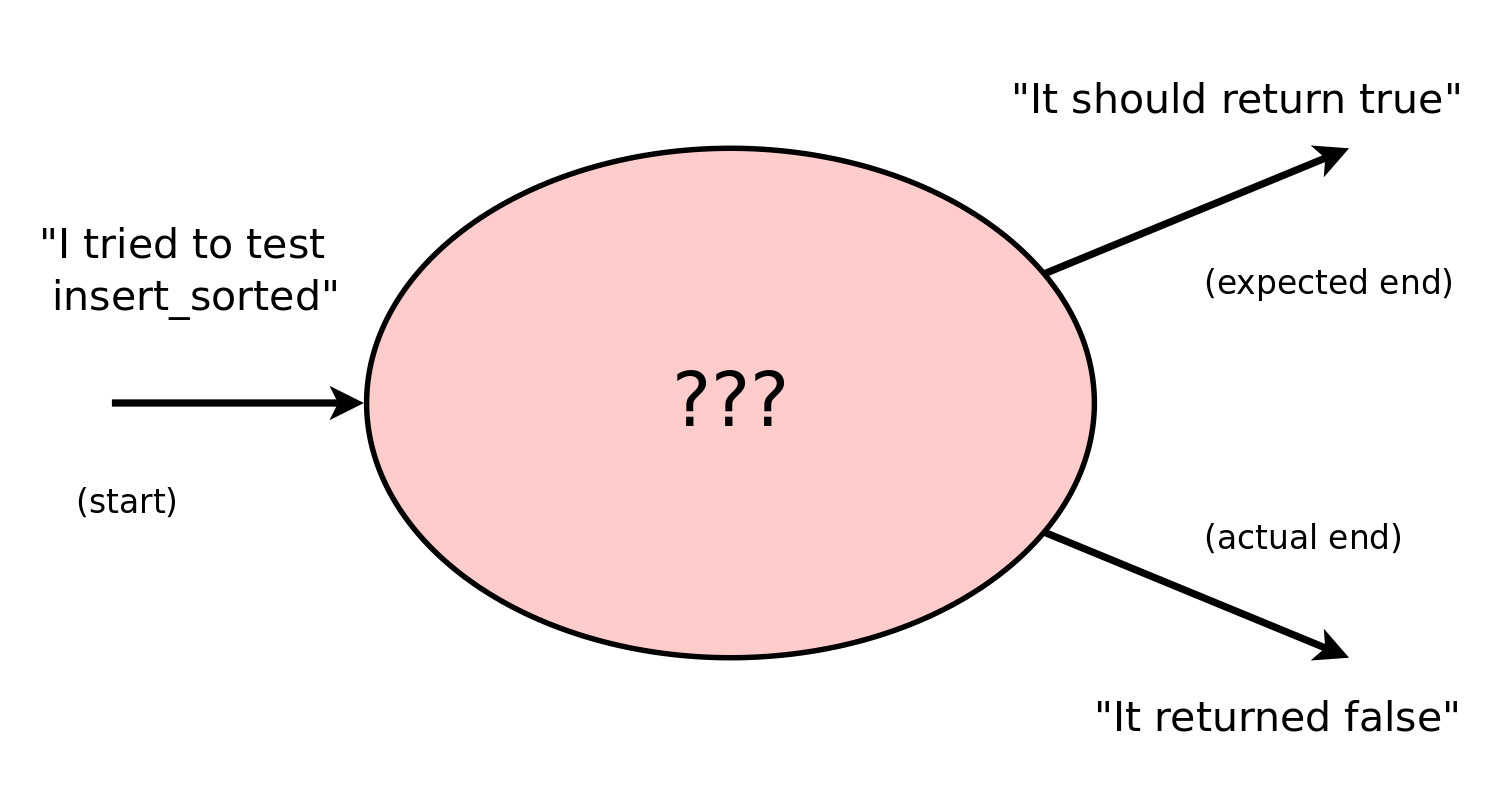
\includegraphics[width=\textwidth]{time0.png}
\end{frame}

\begin{frame}{Print Debugging}
	Make your program print its state during the big pink ``???''.
	\begin{itemize}
		\item Reduce how much of the story the ``???'' obscures.
		\begin{itemize}
			\item Find the {\em last} print {\em before} the bug
			\item Find the {\em first} print {\em after} the bug
		\end{itemize}
	\end{itemize}
	\pause

	\linegap
		\texttt{~~~~\hilight{brown}{foreach}~element~\hilight{brown}{in}~input~\{} \\
		\texttt{~~~~~~~~\hilight{olivegreen}{print(output);}} \\
		\texttt{~~~~~~~~insert\_sorted(output,~element);} \\
		\texttt{~~~~\}} \\
\end{frame}

\begin{frame}{Print Debugging}
	New story:

	\linegap
	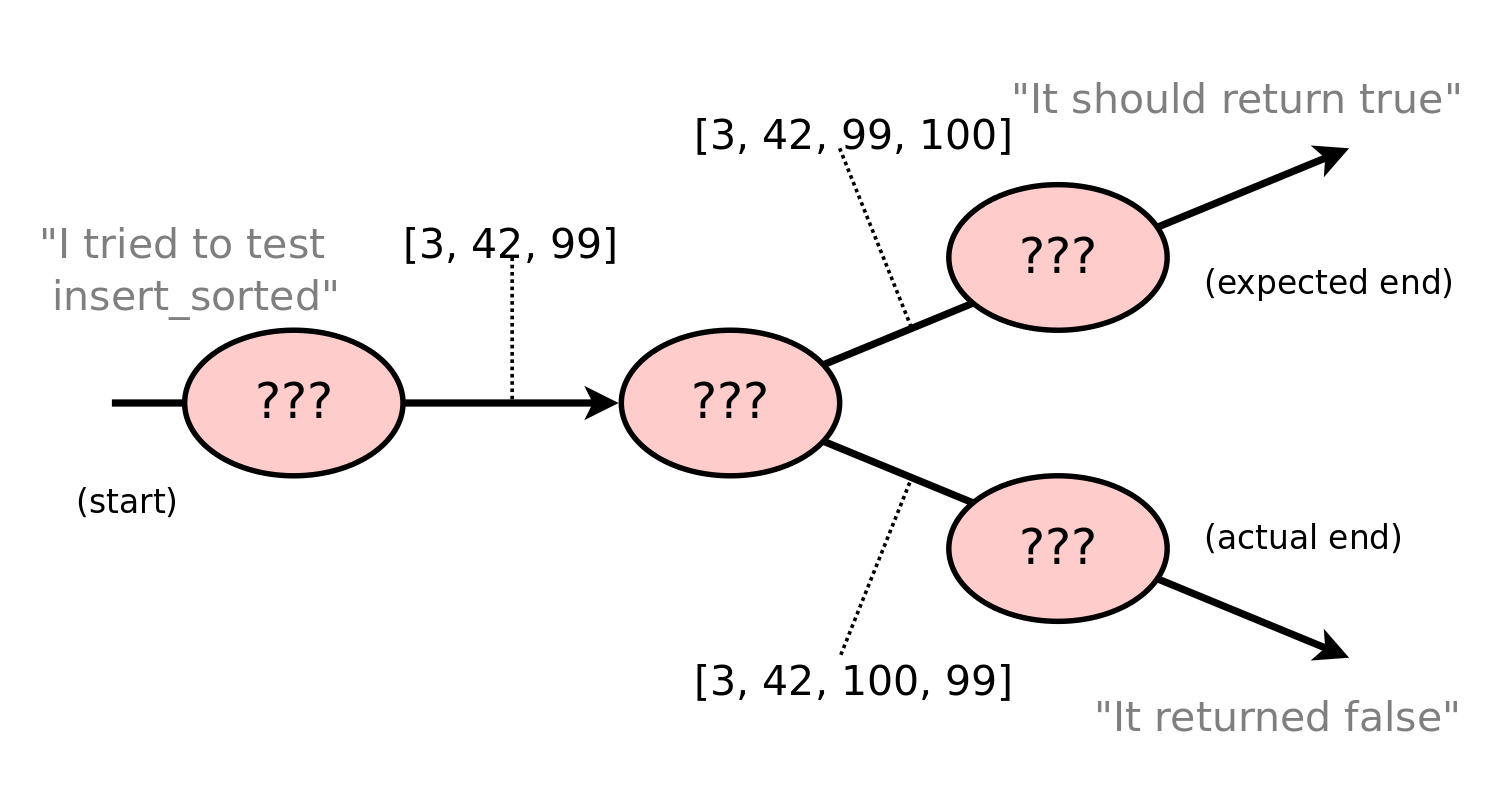
\includegraphics[width=\textwidth]{time1.png}
\end{frame}

\begin{frame}{Asserts: Stealthier, more concealable prints}
\end{frame}

\begin{frame}{Aside: 15-213 ``malloc lab''}
	At the end of 15-213, you will implement \texttt{malloc()}.
	\begin{itemize}
		\item Complex, low-level systems code
		\item Very easy to end up with difficult, subtle bugs
		\begin{itemize}
			\item Your data winds up in the wrong place, gets clobbered by client code
			\item Stale pointers that point to nonsense memory
		\end{itemize}
		\item Your code won't even misbehave immediately, only ``later''.
	\end{itemize}
	\pause
	\linegap

	The assignment will ask you to write a {\bf heap checker}.
	\begin{itemize}
		\item In essence, a very powerful \texttt{assert} for your code.
		\item Debugging and asserts are friends!
	\end{itemize}
\end{frame}

\begin{frame}{Aside: 15-213 ``malloc lab''}
	Many students think: ``I just want to write \texttt{malloc()}. I can do the heap checker later.''
	\pause
	\begin{itemize}
		\item Think of it like a C0 contract that must hold forever.
		\item \textbf{Write the heap checker simultaneously!}
			\pause
			\begin{itemize}
				\item Save time/effort debugging everything else
				\item Your debugging skill will level up
				\item Ben jumps up and down for emphasis
			\end{itemize}
	\end{itemize}
\end{frame}

\subsection{Space Travel}

\breakslide{{\bf Where} things go wrong\dots}

\begin{frame}{Telling a Story of Space}
	Remember, two stories: Expected outcome vs Actual outcome

	\linegap
\end{frame}

%%%%%%%%%%%%%%%%%%%%%%%%%%%%%%%%%%%%%%%%%%%%%%%%%%%%%%%%%%%%%%%%%%%%%%%%%%%%%%%%
\section{Main Approach}
%%%%%%%%%%%%%%%%%%%%%%%%%%%%%%%%%%%%%%%%%%%%%%%%%%%%%%%%%%%%%%%%%%%%%%%%%%%%%%%%

\end{document}
%%%%%%%%%%%%%%%%%%%%%%%%%%%%%%%%%%%%%%%%%%%%%%%%%%%%%%%%%%%%%%%%%%%%%%%%%%%%%%%%
% vim: foldmethod=indent
